%!TEX root = main.tex

\section{Adaptive exploration with a three-level disclosure policy}
\label{sec:3level}

The two-level policy from the previous section implements the explore-then-exploit paradigm using a basic design with parallel full-disclosure paths. The next challenge is to implement \emph{adaptive exploration}, and go below the $T^{2/3}$ barrier. We accomplish this using a construction that adds a middle level to the info-graph. This construction also provides intuition for the main result, the multi-level construction presented in the next section. For simplicity, we assume $K=2$ arms.

For the sake of intuition, consider the framework of bandit algorithms with limited adaptivity. Suppose a bandit algorithm outputs a distribution $p_t$ over arms in each round $t$, and the arm $a_t$ is then drawn independently from $p_t$. This distribution can change only in a small number of rounds, called \emph{adaptivity rounds}, that need to be chosen by the algorithm in advance. A single round of adaptivity corresponds to explore-then-exploit paradigm. Our goal here is to implement one extra adaptivity round, and this is what the middle level accomplishes.


\begin{construction}
The \emph{three-level policy} is defined as follows. The info-graph consists of three levels: the first two correspond to \emph{exploration}, and the third implements \emph{exploitation}. Like in the two-level policy, the first level consists of multiple full-disclosure paths of length $\fdpL$ each, and each agent $t$ in the exploitation level sees full history from exploration  (see Figure~\ref{fig:3level}).

The middle level consists of $N_2$ disjoint subsets of $T_2$ agents each, called \emph{second-level groups}. Each second-level group $S$ has the following property:
\begin{align}\label{eq:group-defn}
\text{all nodes in $S$ are connected to the same nodes outside of $S$, but not to one another.}
\end{align}

\jmcomment{$N_2$ is also used in Lemma 3.6. We need to find another notation. And I think it should be something without subscript 2. It's generally a property of the whole construction. How about $\sigma$.}

The full-disclosure paths in the first level are also split into $N_2$ disjoint subsets, called \emph{first-level groups}. Each first-level group consists of $T_1$ full-disclosure paths, for the total of $T_1\cdot N_2\cdot \fdpL$ rounds in the first layer. There is a 1-1 correspondence between first-level groups $S_1$ and second-level groups $S_2$, whereby each agent $t\in S_2$ observes the full history from the corresponding group $S_1$. More formally, agent $t$ is connected to the last node of each full-disclosure path in $S_1$. In other words, this agent receives message
    $m_t = \SubH{V(S_1)}$,
where $V(S_1)$ is the set of all rounds in $S_1$.
\end{construction}

\begin{figure}[t]
\centering
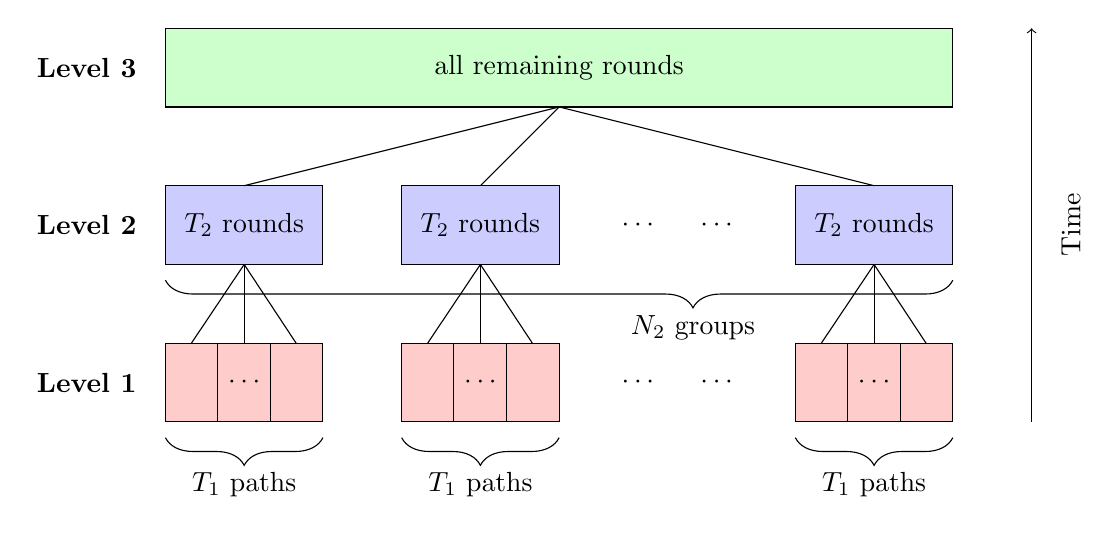
\begin{tikzpicture}
 \filldraw[fill=green!20!white]
 (0,4)--(10,4)--(10,5)--(0,5)--cycle;
 \foreach \x in {0,3,8}
 {
 \filldraw[fill=blue!20!white]
 (\x+0,2)--(\x+2,2)--(\x+2,3)--(\x+0,3)--cycle;
 \draw (\x+1,3)--(5,4);
 \filldraw[fill=red!20!white]
 (\x+0,0)--(\x+2,0)--(\x+2,1)--(\x+0,1)--cycle;
 \draw (\x+1,1)--(\x+1,2);
 \draw(\x+0.33,1)--(\x+1,2);
 \draw(\x+1.66,1)--(\x+1,2);
 %\draw(\x+1.4,1)--(\x+1,2);
 %\draw(\x+1.8,1)--(\x+1,2);
 \draw(\x+0.66,0)--(\x+0.66,1);
 \draw(\x+1.33,0)--(\x+1.33,1);
% \draw (\x+1.2,0)--(\x+1.2,1);
 %\draw(\x+1.6,0)--(\x+1.6,1);
 \node at(\x+1,2.5){$T_2$ rounds};
 \node at(\x+0.33, 0.5){$\GdT$};
 %\node at(\x+0.6, 0.5){$\cdot$};
 \node at(\x+1.0, 0.5){$\cdots$};
 %\node at(\x+1.4, 0.5){$\cdot$};
 \node at(\x+1.66, 0.5){$\GdT$};
 %\node at(\x+1,0.5){$T_1 \cdot \GdT$};
 \draw [decorate,decoration={brace,amplitude=10pt},xshift=0pt,yshift=0pt] (\x+2,-0.2) -- (\x+0,-0.2) node [black,midway,yshift=-0.6cm] {$T_1$ paths};
 }
  \node at(5,4.5){all remaining rounds};
  \node at (6,0.5){$\cdots$};
  \node at (7,0.5){$\cdots$};
  \node at (6,2.5){$\cdots$};
  \node at (7,2.5){$\cdots$};
  \node at(-1,0.5){\textbf{Level 1}};
  \node at(-1,2.5){\textbf{Level 2}};
  \node at(-1,4.5){\textbf{Level 3}};
  \draw[->] (11,0)--(11,5);
  \node at(11.5,2.5)[ rotate=90]{Time};

  \draw [decorate,decoration={brace,amplitude=10pt,aspect=0.33},xshift=0pt,yshift=0pt] (10,1.8) -- (0,1.8) node [black,pos=0.33,xshift = 0cm,yshift=-0.6cm] {$N_2$ groups};

\end{tikzpicture}
\caption{Info-graph for the three-level policy. Each red box in level 1 corresponds to $T_1$ full-disclosure paths of length $\GdT$ each.}
\label{fig:3level}
\end{figure}

The key idea is as follows. Consider the gap parameter $\Delta = |\mu_1-\mu_2|$. If it is is large, then each first-level group produces enough data to determine the best arm with high confidence, and so each agent in the upper levels chooses the best arm. If $\Delta$ is small, then due to \emph{anti-concentration} each arm gets ``lucky" within  at least once first-level group, in the sense that it appears much better than the other arm based on the data collected in this group (and therefore this arm gets explored by the corresponding second-level group). To summarize, the middle level exploits if the gap parameter is large, and provides some more exploration if it is small.

\begin{theorem}
\label{thm:3level}
For two arms, the three-level policy
achieves regret
\[ \reg(T) \leq O\left( T^{4/7}\, \log T \right).\]
This is achieved with parameters
    $T_1 = T^{4/7}\log^{-1/7}(T)$,
    $N_2 = 2^{10}\log(T)$, and
    $T_2 = T^{6/7}\log^{-5/7}(T)$.
\end{theorem}

Let us sketch the proof of this theorem; the full proof can be found in Appendix~\ref{sec:3level-pfs}.

\xhdr{The ``good events".}
We establish four ``good events" each of which occurs with high probability.
\begin{description}
\item[(\event{1})] \emph{Exploration in Level 1:} Every first-level group collects at least $\Omega(T_1)$ samples of each arm.
\item[(\event{2})] \emph{Concentration in Level 1:} Within each first-level group, empirical mean rewards of each arm $a$ concentrate around $\mu_a$.
\item[(\event{3})] \emph{Anti-concentration in Level 1:} For each arm, some first-level subgroup collects data which makes this arm look much better than the other.
\item[(\event{4})] \emph{Concentration in prefix:}
The empirical mean reward of each arm $a$ concentrates around $\mu_a$ in any prefix of its pulls. (This ensures accurate reward estimates in exploitation.)
\end{description}

The analysis of these events applies Chernoff Bounds to a suitable version of ``reward tape" (see the definition of ``reward tape" in Section~\ref{sec:model}). For example, \event{2} considers a reward tape restricted to a given first-level group.

\xhdr{Case analysis.}
We now proceed to bound the regret conditioned on the four ``good events". W.l.o.g., assume $\mu_1 \geq \mu_2$. We break down the regret analysis into four cases, based on the magnitude the gap parameter $\Delta = \mu_1-\mu_2$. As a shorthand, denote
    $\conf{n} = \sqrt{\log(T)/n}$.
In words, this is a confidence term, up to constant factors, for $n$ independent random samples.

The simplest case is very small gap, which trivially yields an upper bound on regret.

\begin{claim}[Negligible gap]
If
%  $\Delta \leq 3\sqrt{\frac{2\log(T)}{T_2}}$,
    $\Delta \leq 3\sqrt{2}\cdot  \conf{T_2}$
then 
  $\reg(T)\leq O(T^{4/7} \log^{6/7}(T))$.
\end{claim}

Another simple case is when $\Delta$ is sufficiently large, so that
the data collected in any first-level group suffices to determine the best arm. The proof follows from \event{1} and \event{2}.

\begin{lemma}[Large gap]\label{3levelbigcase}
If
% $\Delta \geq 2\left(\sqrt{\frac{4\log(T)}{\fdpN[1]T_1}} +
%  \sqrt{\frac{4\log(T)}{\fdpN[2]T_1}}\right)$, 
  $ \Delta \geq 4 \sum_{a\in\A}\; \conf{\fdpN[a]\cdot T_1}$
then all agents in Levels 2 and 3 pull arm 1.
\end{lemma}

In the \emph{medium gap} case, the data collected in a given first-level group is no longer guaranteed to determine the best arm. However, the data collected by the second-level groups enables all agents in the third level to correctly identify the best arm. 

%(even though one of the arms may not be pulled at all in the second level).

\begin{lemma}[Medium gap]\label{3levelmedium}
  All agents pull arm 1 in the third level, when $\Delta$ satisfies
%  \[
%  \Delta\in \left[
%   2\left(\sqrt{\frac{4\log(T)}{S\fdpN[1]T_1}} +
%    \sqrt{\frac{4\log(T)}{S\fdpN[2]T_1}}\right),
% 2\left(\sqrt{\frac{4\log(T)}{\fdpN[1]T_1}} +
%        \sqrt{\frac{4\log(T)}{\fdpN[2]T_1}}\right),
%    \right)
%  \]
\[ \textstyle \Delta\in \left[
    4\,\sum_{a\in\A}\; \conf{N_2\cdot \fdpN[a]\cdot T_1},\quad
    4\,\sum_{a\in\A}\; \conf{\fdpN[a]\cdot T_1}
 \right] \]
\end{lemma}


Finally, the \emph{small gap} case, when  $\Delta$ is between
$\tilde\Omega(\sqrt{1/T_2})$ and $\tilde O(\sqrt{1/(N_2\, T_1)})$ 
is more challenging since even aggregating the data from all $N_2$
first-level groups is not sufficient for identify the best arm. 
We need to ensure that both arms continue to be explored in the second level. 
To achieve this, we leverage \event[4], which implies 
that each arm $a$ has a first-level group $s_a$ where it gets ``lucky", in the sense that its empirical mean reward is slightly higher than $\mu_a$, while the empirical mean reward of the other arm is slightly lower than its true mean. Since the
deviations are in the order of $\Omega(\sqrt{1/T_1})$, and Assumption~\ref{ass:embehave} guarantees the agents' reward estimates are also within $\Omega(\sqrt{1/T_1})$ of the empirical means, the sub-history
from this group $s_a$ ensures that all agents in the respective second-level group prefer arm $a$. Therefore, both arms are pulled at least $T_2$ times in the second level, which in turn gives the following guarantee:


\begin{lemma}[Small gap]\label{3levelsmallcase}
  All agents pull arm 1 in the third level, when $\Delta$ satisfies
%  \[
%    \Delta\in \left( 3\sqrt{\frac{2\log(T)}{T_2}},
%      2\left(\sqrt{\frac{4\log(T)}{S \fdpN[1]T_1}} +
%        \sqrt{\frac{4\log(T)}{S \fdpN[2]T_1}}\right) \right)
%  \]
\[ \textstyle 
    \Delta\in \left( 3\sqrt{2}\cdot\conf{T_2},\quad
      4\,\sum_{a\in\A}\; \conf{N_2\cdot \fdpN[a]\cdot T_1}
\right)
\]
\end{lemma}


\paragraph{Wrapping up: proof of \Cref{thm:3level}. } In negligible
gap case, the stated regret bound holds regardless of what the algorithm does. In the large gap case, the regret only comes from the
first level, so it is upper-bounded by the total number of agents in this level, which is 
    $N_2\cdot \GdT \cdot T_1 = O(T^{4/7} \log T)$. 
In both intermediate cases, it suffices to bound the regret from the
first and second levels, so
\[ \textstyle 
\reg(T) \leq (N_2\,T_1\cdot \GdT + N_2\, T_2) 
\cdot 4\,\sum_{a\in\A}\; \conf{\fdpN[a]\cdot T_1}
= O(T^{4/7} \log^{6/7}(T)).
\]
Therefore, we obtain the stated regret bound in all cases.




\OMIT{
\begin{proof}
Wlog we assume $\mu_1 \geq \mu_2$ as the recommendation policy is symmetric to both arms. We do a case analysis based on $\mu_1-\mu_2$.

Before we start with the case analysis, we first define several clean events and show that the intersection of them happens with high probability.

\begin{itemize}

\item \textbf{Concentration of the number of arm $a$ pulls in the first level:}
\OMIT{By Lemma \ref{lem:greedy}, we know $\GdP \leq \fdpN  \leq \GdT$. For the $s$-th first-level group, define $W_1^{a,s}$ to be the event that the number of arm $a$ pulls in the $s$-th first-level group is between $\fdpN  T_1- \GdT \sqrt{T_1\log(T)}$ and $\fdpN  T_1 + \GdT \sqrt{T_1\log(T)}$. By Chernoff bound,}
For the $s$-th first-level group, define $W_1^{a,s}$ to be the event
that the number of arm $a$ pulls in the $s$-th first-level group is
between $\fdpN  T_1- \GdT \sqrt{T_1\log(T)}$ and
$\fdpN  T_1 + \GdT \sqrt{T_1\log(T)}$. By Lemma~\ref{lem:t1runs}
\[
\Pr[W_1^{a,s}] \geq 1-2\exp(-2\log(T)) \geq 1-2/T^2.
\]
Let $W_1$  be the intersection of all these events (i.e.
$W_1 = \bigcap_{a,s}W_1^{a,s}$). By union bound, we have
\[
\Pr[W_1] \geq 1- \frac{4S}{T^2}.
\]}

\OMIT{\item \textbf{Concentration of the empirical mean of arm $a$ pulls in the first level:}
For each first-level group and arm $a$, imagine there is a tape of enough arm $a$ pulls sampled before the recommendation policy starts and these samples are revealed one by one whenever agents in this group pull arm $a$. For the $s$-th first-level group and arm $a$, define $W_2^{s,a,t_1,t_2}$ to be the event that the mean of $t_1$-th to $t_2$-th pulls in the tape is at most $\sqrt{\frac{2\log(T)}{t_2-t_1+1}}$ away from $\mu_a$. By Chernoff bound,\swcomment{a bit confused about what $t_1$ and $t_2$ mean?}
\[
\Pr[W_2^{s,a,t_1,t_2}] \geq 1 - 2\exp(-4\log(T)) \geq 1- 2/T^4.
\]

Define $W_2$ to be the intersection of all these events (i.e. $W_2 = \bigcap_{a,s,t_1,t_2} W_2^{s,a,t_1,t_2}$). By union bound, we have
\[
\Pr[W_2] \geq 1- \frac{4S}{T^2}.
\]
}
\OMIT{\item \textbf{Concentration of the empirical mean of arm $a$ pulls in the first two levels:}

For all the groups in the first two levels and arm $a$, imagine there is a tape of enough arm $a$ pulls sampled before the recommendation policy starts and these samples are revealed one by one whenever agents in the first two levels pull arm $a$. Define $W_3^{a,t}$ to be the event that the mean of the first $t$ pulls in the tape is at most $\sqrt{\frac{2\log(T)}{t}}$ away from $\mu_a$. By Chernoff bound,
\[
\Pr[W_3^{a,t}] \geq 1 - 2\exp(-4\log(T)) \geq 1- 2/T^4.
\]
Define $W_3$ to be the intersection of all these events (i.e. $W_3 = \bigcap_{a,t} W_3^{a,t}$). By union bound, we have
\[
\Pr[W_3] \geq 1- \frac{4}{T^3}.
\]
}
\OMIT{\item \textbf{Anti-concentration of the empirical mean of arm $a$ pulls in the first level:}

Consider the tapes defined in the second bullet again. For the $s$-th first-level group and arm $a$, define $W_4^{s,a,high}$  to be the event that first $\fdpN  T_1$ pulls of arm $a$ in the corresponding tape has empirical mean at least $\mu_a + 1/\sqrt{\fdpN  T_1}$ and define  $W_4^{s,a,low}$  to be the event that first $\fdpN  T_1$ pulls of arm $a$ in the corresponding tape has empirical mean at most $\mu_a - 1/\sqrt{\fdpN  T_1}$. By Berry-Essen Theorem and $\mu_a \in [1/3,2/3]$, we have
\[
\Pr[W_4^{s,a,high}] \geq (1-\Phi(1/2)) - \frac{5}{\sqrt{\fdpN T_1}} > 1/4.
\]
The last inequality follows when $T$ is larger than some constant.
Similarly we also have
\[
\Pr[W_4^{s,a,low}] > 1/4.
\]
Since $W_4^{s,a,high}$ is independent with $W_4^{s,3-a,low}$, we have
\[
\Pr[W_4^{s,a,high} \cap W_4^{s,3-a,low}] =\Pr[W_4^{s,a,high}] \cdot  \Pr[W_4^{s,3-a,low}]>(1/4)^2 = 1/16.
\]
Now define $W_4$ as $\bigcap_a \bigcup_s (W_4^{s,a,high} \cap W_4^{s,3-a,low})$. Notice that $(W_4^{s,a,high} \cap W_4^{s,3-a,low})$ are independent across different $s$'s. By union bound, we have
\[
\Pr[W_4] \geq 1- 2(1-1/16)^S \geq 1 -2 /T.
\]
\end{itemize}

By union bound, the intersection of these clean events (i.e. $\bigcap_{i=1}^4 W_i$) happens with probability $1-O(1/T)$. When this intersection does not happen, since the probability is $O(1/T)$, it contributes $O(1/T) \cdot T = O(1)$ to the expected regret.

Now we assume the intersection of clean events happens and we summarize what these clean events imply.

\begin{itemize}
\item For the $s$-th first-level group and arm $a$, define $\bar{\mu}_a^{1,s}$ to be the empirical mean of arm $a$ pulls in this group. $W_1^{a,s}$, $W_2^{a,s,1,t}$ for $ = \fdpN  T_1- \GdT \sqrt{T_1\log(T)},...,\fdpN  T_1- \GdT \sqrt{T_1\log(T)}$ together imply that
\[
|\bar{\mu}_a^{1,s} - \mu_a| \leq \sqrt{\frac{2\log(T)}{\fdpN  T_1- \GdT \sqrt{T_1\log(T)}}} \leq \sqrt{\frac{4\log(T)}{\fdpN  T_1}}.
\]
The last inequality holds when $T$ is larger than some constant.
\item For each arm $a$, define $\bar{\mu}_a$ to be the empirical mean of arm $a$ pulls in the first two levels. $W_1^{a,s}$ for $s=1,...,S$ and $W_3^{a,t}$ for $t \geq  (\fdpN  T_1- \GdT \sqrt{T_1\log(T)})S$ together imply that
\[
|\bar{\mu}_a - \mu_a| \leq \sqrt{\frac{2\log(T)}{S\left(\fdpN  T_1- \GdT \sqrt{T_1\log(T)}\right)}} \leq \sqrt{\frac{4\log(T)}{S \fdpN  T_1}} .
\]
The last inequality holds when $T$ is larger than some constant.

If there are at least $T_2$ pulls of arm $a$ in the first two levels,
\[
|\bar{\mu}_a-\mu_a| \leq \sqrt{\frac{2\log(T)}{T_2}}.
\]

\item For each $a \in \{1,2\}$, $W_4$ implies that there exists $s_a$ such that $W_4^{s_a,a,high}$ and $W_4^{s_a,3-a,low}$ happen. $W_4^{s_a,a,high}$,  $W_1^{s_a,a}$, $W_2^{s_a,a,t, \fdpN T_1}$ for $t = \fdpN  T_1- \GdT \sqrt{T_1\log(T)}+1, ...,\fdpN T_1-1$ and $W_2^{s_a,a,\fdpN T_1,t}$ for $t= \fdpN T_1,...,\fdpN  T_1+ \GdT \sqrt{T_1\log(T)}$ together imply that
\begin{align*}
\bar{\mu}_a ^{1,s_a} &\geq \mu_a + \left(\fdpN T_1 \cdot \frac{1}{\sqrt{\fdpN T_1}} - \GdT \sqrt{T_1\log(T)} \cdot \sqrt{\frac{2\log(T)}{ \GdT \sqrt{T_1\log(T)}}} \right) \cdot \frac{1}{\fdpN  T_1+ \GdT \sqrt{T_1\log(T)}} \\
&> \mu_a + \frac{1}{4\sqrt{\fdpN T_1}}.
\end{align*}
The second last inequality holds when $T$ is larger than some constant.
Similarly, we also have
\[
\bar{\mu}_{3-a} ^{1,s_a} < \mu_{3-a}   - \frac{1}{4\sqrt{q_{3-a} T_1}}.
\]
\end{itemize}

Finally we proceed to the case analysis. We give upper bounds on the expected regret conditioned on the intersection of clean events.

\begin{itemize}

\item $\mu_1 - \mu_2 \geq 2\left(\sqrt{\frac{4\log(T)}{\fdpN[1]T_1}}
+ \sqrt{\frac{4\log(T)}{\fdpN[2]T_1}}\right)$. In this case, we want to show that agents in the second and the third levels all pull arm 1.

First consider the $s$-th second-level group. We know that
\[
\bar{\mu}_1^{1,s} - \bar{\mu}_2^{1,s} \geq \mu_1 -\mu_2 - \sqrt{\frac{4\log(T)}{\fdpN[1]T_1}} - \sqrt{\frac{4\log(T)}{\fdpN[2]T_1}} \geq  \sqrt{\frac{4\log(T)}{\fdpN[1]T_1}} + \sqrt{\frac{4\log(T)}{\fdpN[2]T_1}}.
\]
For any agent $t$ in the $s$-th second-level group, by Assumption \ref{ass:embehave}, we have
\begin{align*}
\hat{\mu}_1^t - \hat{\mu}_2^t &>\bar{\mu}_1^{1,s} - \bar{\mu}_2^{1,s} - \frac{c_m}{\sqrt{\fdpN[1]T_1/2}} - \frac{c_m}{\sqrt{\fdpN[2]T_1/2}}\\
&\geq  \sqrt{\frac{4\log(T)}{\fdpN[1]T_1}} + \sqrt{\frac{4\log(T)}{\fdpN[2]T_1}}- \frac{c_m}{\sqrt{\fdpN[1]T_1/2}} - \frac{c_m}{\sqrt{\fdpN[2]T_1/2}}\\
 &> 0.
\end{align*}
Therefore, we know agents in the $s$-th second-level group will all pull arm 1.

Now consider the agents in the third level group. Recall $\bar{\mu}_a$ is the empirical mean of arm $a$ in the history they see. We have
\[
\bar{\mu}_1 - \bar{\mu}_2 \geq \mu_1 -\mu_2 - \sqrt{\frac{4\log(T)}{S\fdpN[1]T_1}} - \sqrt{\frac{4\log(T)}{S\fdpN[2]T_1}} \geq  \sqrt{\frac{4\log(T)}{\fdpN[1]T_1}}
+ \sqrt{\frac{4\log(T)}{\fdpN[2]T_1}}.
\]
Similarly as above, by Assumption \ref{ass:embehave}, we know $\hat{\mu}_1^t - \hat{\mu}_2^t > 0$ for any agent $t$ in the third level. So we know agents in the third-level group will all pull arm 1. Therefore the expected regret is at most $S T_G T_1 = O(T^{4/7} \log^{6/7}(T))$.


\item $2\left(\sqrt{\frac{4\log(T)}{S\fdpN[1]T_1}}
+ \sqrt{\frac{4\log(T)}{S\fdpN[2]T_1}}\right) \leq \mu_1-\mu_2 < 2\left(\sqrt{\frac{4\log(T)}{\fdpN[1]T_1}}
+ \sqrt{\frac{4\log(T)}{\fdpN[2]T_1}}\right)$. In this case, we want to show agents in the third level all pull arm 1. Recall $\bar{\mu}_a$ is the empirical mean of arm $a$ in the first two levels. We have
\[
\bar{\mu}_1 - \bar{\mu}_2 \geq \mu_1 -\mu_2 - \sqrt{\frac{4\log(T)}{S\fdpN[1]T_1}} - \sqrt{\frac{4\log(T)}{S\fdpN[2]T_1}} \geq  \sqrt{\frac{4\log(T)}{S\fdpN[1]T_1}}
+ \sqrt{\frac{4\log(T)}{S\fdpN[2]T_1}}.
\]
For any agent $t$ in the third level, by Assumption \ref{ass:embehave}, we have
\begin{align*}
\hat{\mu}_1^t - \hat{\mu}_2^t &>\bar{\mu}_1 - \bar{\mu}_2 - \frac{c_m}{\sqrt{S\fdpN[1]T_1/2}} - \frac{c_m}{\sqrt{S\fdpN[2]T_1/2}}\\
&\geq  \sqrt{\frac{4\log(T)}{S\fdpN[1]T_1}} + \sqrt{\frac{4\log(T)}{S\fdpN[2]T_1}}- \frac{c_m}{\sqrt{S\fdpN[1]T_1/2}} - \frac{c_m}{\sqrt{S\fdpN[2]T_1/2}}\\
 &> 0.
\end{align*}
So we know agents in the third-level group will all pull arm 1. Therefore the expected regret is at most
\[
(S T_G T_1 + S T_2) \cdot 2\left(\sqrt{\frac{4\log(T)}{\fdpN[1]T_1}}
+ \sqrt{\frac{4\log(T)}{\fdpN[2]T_1}}\right) = O(T^{4/7} \log^{6/7}(T))
\]

\item $ 3\sqrt{\frac{2\log(T)}{T_2}} < \mu_1-\mu_2 < 2\left(\sqrt{\frac{4\log(T)}{S\fdpN[1]T_1}}
+ \sqrt{\frac{4\log(T)}{S\fdpN[2]T_1}}\right)$. In this case, we just need to make sure that agents in the third level all pull arm 1. To do so, we need both arms to be pulled at least $T_2$ rounds in the second level.

Now consider the $s_a$-th second-level group. We have
\begin{align*}
\bar{\mu}_a^{1,s_a} - \bar{\mu}_{3-a}^{1,s_a} &> \mu_a + \frac{1}{4\sqrt{\fdpN T_1}} -\mu_{3-a} +\frac{1}{4\sqrt{q_{3-a}T_1}} \\
&> \frac{1}{4\sqrt{\fdpN[1]T_1}}+ \frac{1}{4\sqrt{\fdpN[2]T_1}} - 2\left(\sqrt{\frac{4\log(T)}{S\fdpN[1]T_1}}
+ \sqrt{\frac{4\log(T)}{S\fdpN[2]T_1}}\right) \\
&\geq \frac{1}{8\sqrt{\fdpN[1]T_1}}+ \frac{1}{8\sqrt{\fdpN[2]T_1}}.
\end{align*}
For any agent $t$ in the $s_a$-th second-level group, by Assumption \ref{ass:embehave}, we have
\begin{align*}
\hat{\mu}_a^t - \hat{\mu}_{3-a}^t &>\bar{\mu}_a^{1,s_a} - \bar{\mu}_{3-a}^{1,s_a} - \frac{c_m}{\sqrt{\fdpN[1]T_1/2}} - \frac{c_m}{\sqrt{\fdpN[2]T_1/2}}\\
&\geq   \frac{1}{8\sqrt{\fdpN[1]T_1}}+ \frac{1}{8\sqrt{\fdpN[2]T_1}}- \frac{c_m}{\sqrt{\fdpN[1]T_1/2}} - \frac{c_m}{\sqrt{\fdpN[2]T_1/2}}\\
 &> 0.
\end{align*}
So we know agents in the $s_a$-th second-level group will all pull arm $a$. Therefore in the first two levels, both arms are pulled at least $T_2$ times. Now consider the third-level. We have
\[
\bar{\mu}_1 - \bar{\mu}_2  \geq \mu_1 -\mu_2 - 2\sqrt{\frac{2\log(T)}{T_2}} \geq \sqrt{\frac{2\log(T)}{T_2}}.
\]
Similarly as above, by Assumption \ref{ass:embehave}, we know $\hat{\mu}_1^t - \hat{\mu}_2^t > 0$ for any agent $t$ in the third level. So we know agents in the third-level group will all pull arm 1.

Therefore the expected regret is at most
\[
(S T_G T_1 + S T_2) \cdot 2\left(\sqrt{\frac{4\log(T)}{S\fdpN[1]T_1}}
+ \sqrt{\frac{4\log(T)}{S\fdpN[2]T_1}}\right) \leq O(T^{4/7} \log^{6/7}(T))
\]


\item $\mu_1 - \mu_2 \leq 3\sqrt{\frac{2\log(T)}{T_2}}$. This is the easy case. Even always pulling the sub-optimal arm (i.e. arm 2) gives regret at most $T \cdot (\mu_1-\mu_2) = O(T^{4/7} \log^{6/7}(T))$.
\end{itemize}
\end{proof}}

%%% Local Variables:
%%% mode: latex
%%% TeX-master: "main"
%%% End:
